\section*{TCP: Tcpdump}
A tcpdump packet capture was started and the scan written to a WireShark compatible pcap file for analysis. The tcpdump terminal output is shown in Listing~\ref{list:tcp_tcpdump}. The Ncat terminal output where the group member's names and MAC ID numbers were echoed is shown below in Listing~\ref{list:echo}.

\begin{lstlisting}[caption=Tcpdump Packet Capture of Python Echo Server Connection,label=list:tcp_tcpdump]
sudo tcpdump -nnvvX -i 1 -S host compeng4dn4.mooo.com -w mooo_echo.pcap
tcpdump: listening on eth0, link-type EN10MB (Ethernet), snapshot length 262144 bytes
21 packets captured
88 packets received by filter
0 packets dropped by kernel
\end{lstlisting}

\begin{lstlisting}[caption=Ncat Connection to Python Echo Server,label=list:echo]
ncat --crlf compeng4dn4.mooo.com 50007
Wecome to COMPENG 4DN4 Echo Server!
Raeed Hassan
Raeed Hassan
400188200
400188200
Aaron Pinto
Aaron Pinto
400190637
400190637
\end{lstlisting}

The capture displayed in WireShark is shown below in Figure~\ref{fig:echo_wireshark}.

\begin{figure}[htp]
\centering
\caption[echo_wireshark]{Tcpdump Capture of Python Echo Server in WireShark}\label{fig:echo_wireshark}
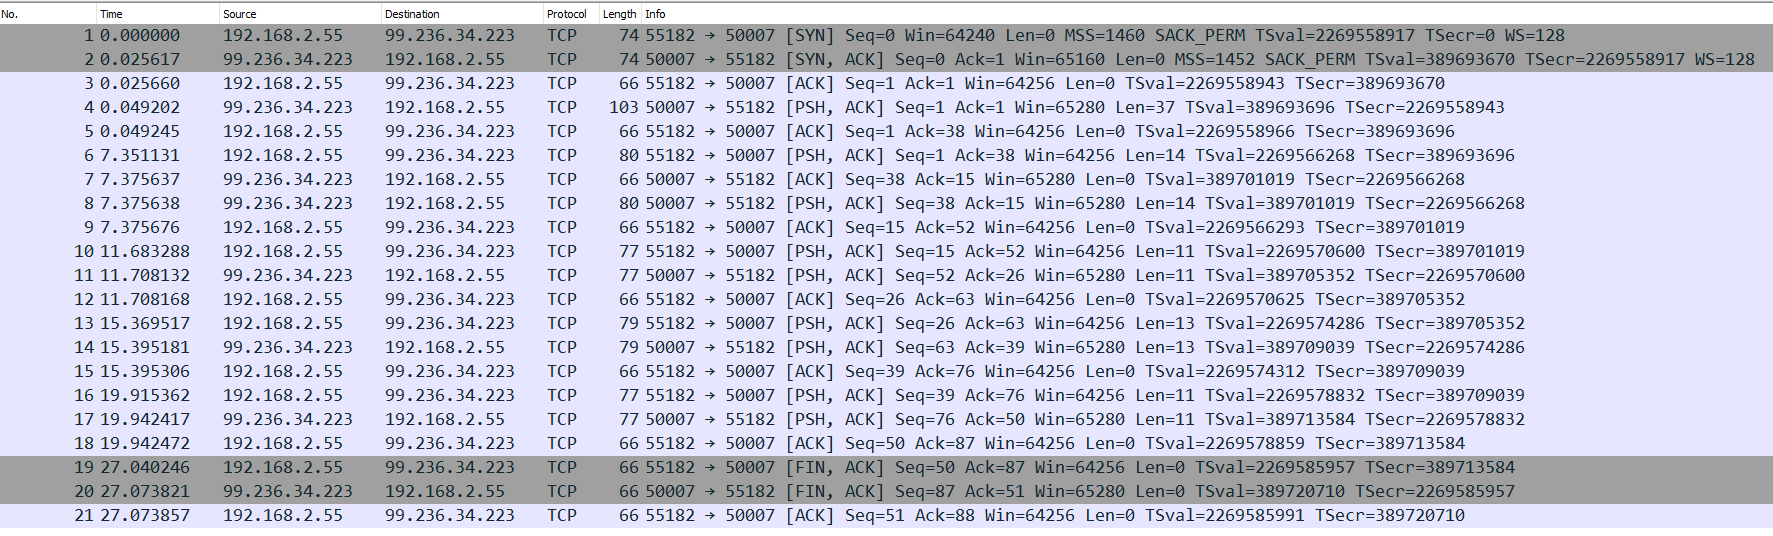
\includegraphics[width=\textwidth]{echo_server.png}
\end{figure}